\documentclass[11pt,a4paper]{article}
\usepackage[a4paper,margin=2.3cm]{geometry}
\usepackage[T1]{fontenc}
\usepackage{lmodern}
\usepackage{microtype}
\usepackage{booktabs}
\usepackage{tabularx}
\usepackage{siunitx}
\usepackage{graphicx}
\usepackage{xcolor}
\usepackage{tikz}
\usetikzlibrary{positioning,arrows.meta,fit,backgrounds,calc}
\usepackage{enumitem}
\usepackage{caption}
\usepackage{float}
\usepackage{needspace}
\usepackage[raggedright]{titlesec}
\usepackage[hidelinks]{hyperref}

\sisetup{group-separator={,},group-minimum-digits=4}
\setlist{nosep,leftmargin=1.2em}
\captionsetup{font=small,labelfont=bf}
\setlength{\parskip}{3pt}
\newcommand{\code}[1]{\texttt{\small #1}}
\newcolumntype{L}{>{\raggedright\arraybackslash}X}

% no paragraph may leave 3 lines or fewer alone at the bottom or top of a page
\clubpenalties 4 10000 10000 10000 0
\widowpenalties 4 10000 10000 10000 0
\raggedbottom
% let floats share pages with text, and put float pages at the top instead of centring them
\renewcommand{\topfraction}{0.85}
\renewcommand{\bottomfraction}{0.6}
\renewcommand{\textfraction}{0.1}
\renewcommand{\floatpagefraction}{0.8}
\makeatletter
\setlength{\@fptop}{0pt}
\setlength{\floatsep}{24pt plus 4pt minus 4pt}
\setlength{\textfloatsep}{18pt plus 4pt minus 4pt}
\makeatother
% a heading needs room for itself and at least four lines of text, otherwise it moves to the next page
\newcommand{\sectionbreak}{\Needspace{7\baselineskip}}
\newcommand{\subsectionbreak}{\Needspace{6\baselineskip}}

\title{Did the pandemic and e-bikes change\\ how New Yorkers use Citi Bike?\\[4pt]
\large A Medallion pipeline over 334 million trips from 2013 to 2026}
\author{Alexander Rebello \\ DAT535 Data Engineering, University of Stavanger \\[10pt]
\small Code: \url{https://github.com/alexander-rebello/citibike-medallion} \\
\small Dashboard: \url{https://alexander-rebello.github.io/citibike-medallion/}}
\date{November 2026}

\begin{document}
\maketitle

% ---------------------------------------------------------------------------------------------
\section{Question and consumer}

Citi Bike is the bike sharing system of New York City and publishes every trip since June 2013. After 2019 two events
changed the conditions for the system. The first was the COVID-19 pandemic in 2020, the second was the move to an electric
fleet, which today carries most of the trips. This project asks whether these two events changed how New Yorkers use the
system. The intended consumer is a city planner or the operator itself, so every number in the answer has to be traceable
back to the raw data.

Four measures were agreed with the supervisor before any code was written:
\begin{enumerate}
\item the share of trips made by casual riders,
\item the daily demand peaks,
\item the trip length on electric bikes compared to classic bikes,
\item whether the busiest start points move away from central Manhattan.
\end{enumerate}
The core comparison uses the years 2015, 2019 and 2024. The pipeline still processes the full history from June 2013 to
October 2026, so that the core years can be seen in context.

The answer in Section~\ref{sec:results} can only be as good as the cleaning of 334 million rows that were written by two
generations of software and use eight different timestamp formats. For this reason the Silver layer takes the most space
in this report.

\newpage
% ---------------------------------------------------------------------------------------------
\section{Understanding the raw data}
\label{sec:data}

The source is a public S3 bucket with yearly zip files for 2013 to 2024 and monthly zip files from 2025 on. Some yearly
archives contain nested folders and macOS metadata files. Files for Jersey City are out of scope. A download script streams
every CSV file into gzip without changing a single byte and writes a manifest with file, month, size, header and row count.
In total there are 161 monthly datasets with \num{333888858} rows.

\subsection{Two schemas and four headers}

The data follows two logical schemas. The legacy schema \code{legacy\_v1} covers June 2013 to December 2019. It has a trip
duration column, a bike id, birth year and gender, and one coordinate pair per station. The modern schema
\code{modern\_v2} starts in January 2020. It has a ride id, the bike type, the rider type member or casual, and coordinates
for every single trip with more than 13 decimals, but no bike id and no demographic data. The legacy schema appears with
three spellings of the header: lower case, quoted, and Title Case between October 2016 and March 2017.

Every header is identified by a fingerprint, which is the start of a SHA-256 hash over the lower case header. The known
fingerprints are kept in a schema registry, and a header that is not registered stops the pipeline
(Section~\ref{sec:ops}).

\subsection{Duplicated file sets}

Nineteen yearly archives contain the same month twice, once as a single file and once split into several parts. For each
of these months I checked that both sets have exactly the same number of rows and kept only one of them. Without this check
these months would have been counted twice.

\subsection{A wrong assumption, corrected by measuring}

An early sample of the January and June files suggested that the timestamp format changes once per year. Before writing
any Silver rule I therefore profiled all 161 months on the cluster, which took 7 minutes and 40 seconds. Every value of
every column was classified by its shape and counted per month. Figure~\ref{fig:formats} shows the result: eight runs of
formats that change from one month to the next, but never within a month. In 2015 the format alternates between timestamps
with and without seconds. January to March and June have no seconds, the other months do. The January and June sample
could not show this, and a rule per year would have failed for part of 2015.

The same profile also found the different styles of station ids, the markers for missing birth years, the service
stations and the coordinate outliers. These findings are the basis for the Silver rules in Table~\ref{tab:rules}.

\begin{figure}[b]
\centering
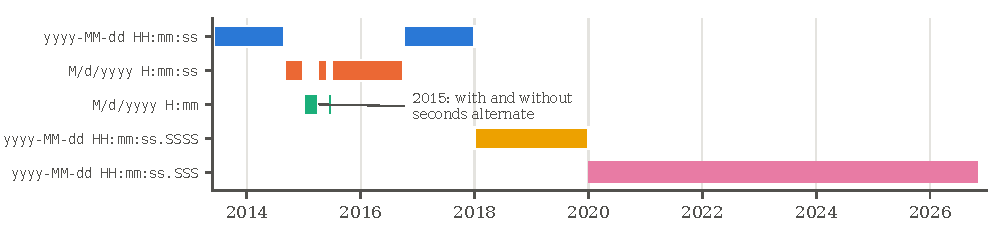
\includegraphics[width=\linewidth]{figures/formats.pdf}
\vspace{-14pt}
\caption{Timestamp format by month, measured over all 161 months. Each run of months gets its own parse pattern in
\code{config/silver\_rules.toml}. Months without seconds take the duration from the \code{tripduration} column.}
\label{fig:formats}
\end{figure}

% ---------------------------------------------------------------------------------------------
\section{Architecture and environments}

The pipeline follows the Medallion architecture and is built on files (Figure~\ref{fig:arch}). Each layer is a set of
Parquet tables, compressed with zstd and partitioned by year and month. Next to the tables every layer keeps a ledger and a
run log in a \code{\_meta} folder. All transformations use the Spark DataFrame API and Spark SQL, and no Python UDFs are
used.

\begin{figure}[hb]
\centering
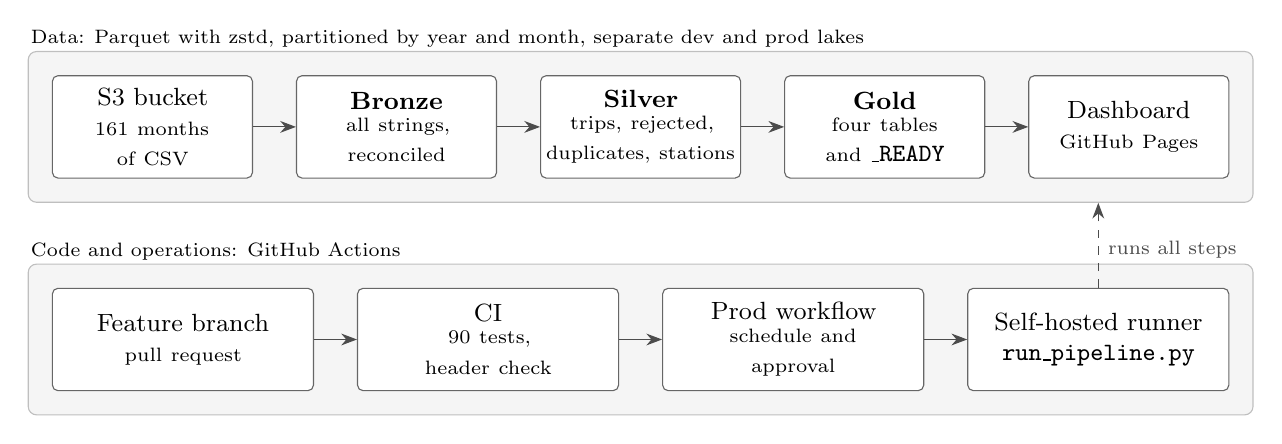
\begin{tikzpicture}[
  font=\small,
  box/.style={draw=black!60, rounded corners=2pt, align=center, minimum height=13mm, fill=white, inner sep=2pt},
  arr/.style={-{Stealth[length=2mm]}, black!70},
  lane/.style={draw=black!25, rounded corners=3pt, fill=black!4},
  lanelabel/.style={font=\scriptsize, anchor=south west, inner sep=1pt}]
% data lane: five boxes of 24 mm with 7 mm gaps (148 mm in total)
\foreach \i/\name/\txt in {0/raw/{S3 bucket\\\scriptsize 161 months of CSV},
                          1/bronze/{\textbf{Bronze}\\\scriptsize all strings,\\\scriptsize reconciled},
                          2/silver/{\textbf{Silver}\\\scriptsize trips, rejected,\\\scriptsize duplicates, stations},
                          3/gold/{\textbf{Gold}\\\scriptsize four tables\\\scriptsize and \code{\_READY}},
                          4/dash/{Dashboard\\\scriptsize GitHub Pages}}
  \node[box, text width=24mm, anchor=west] (\name) at (\i*31mm, 0) {\txt};
\foreach \a/\b in {raw/bronze, bronze/silver, silver/gold, gold/dash} \draw[arr] (\a) -- (\b);
% operations lane: four boxes over the same width
\foreach \i/\name/\txt in {0/git/{Feature branch\\\scriptsize pull request},
                          1/ci/{CI\\\scriptsize 90 tests,\\\scriptsize header check},
                          2/prod/{Prod workflow\\\scriptsize schedule and\\\scriptsize approval},
                          3/run/{Self-hosted runner\\\scriptsize \code{run\_pipeline.py}}}
  \node[box, text width=31.75mm, anchor=west] (\name) at (\i*38.75mm, -27mm) {\txt};
\foreach \a/\b in {git/ci, ci/prod, prod/run} \draw[arr] (\a) -- (\b);
\begin{scope}[on background layer]
  \node[lane, fit={(raw.north west) (dash.south east)}, inner sep=3mm] (dl) {};
  \node[lane, fit={(git.north west) (run.south east)}, inner sep=3mm] (ol) {};
\end{scope}
\node[lanelabel] at (dl.north west) {Data: Parquet with zstd, partitioned by year and month, separate dev and prod lakes};
\node[lanelabel] at (ol.north west) {Code and operations: GitHub Actions};
\draw[arr, dashed] (run.north) -- (run.north |- dl.south) node[pos=0.45, right, font=\scriptsize] {runs all steps};
\end{tikzpicture}
\caption{Architecture of the pipeline. All layers are Parquet files on a shared file system, and Spark runs on a standalone
cluster with two nodes.}
\label{fig:arch}
\end{figure}

\subsection{Development and production}

A single environment variable, \code{CITIBIKE\_ENV}, selects a configuration file and a separate data lake. The development
environment holds six months that were chosen so that every schema, header spelling and timestamp format appears at least
once. A full run on it takes about two minutes. The production environment holds all 161 months, which amounts to 9.6~GB
in Bronze, 14~GB in Silver and 0.36~GB in Gold.

\subsection{Cluster}

The cluster consists of two virtual machines with 8 virtual CPUs and 16~GB of memory each. The main node holds the data,
the Spark master, one worker, the driver and the GitHub Actions runner. The second node runs another worker and mounts the
data lake over NFS at the same path. Master and workers run as systemd services that are configured from the repository,
so the cluster comes back after a reboot and is always set up in the same way. Every Spark job writes an event log, and
these logs are the evidence for Section~\ref{sec:perf}.

% ---------------------------------------------------------------------------------------------
\section{Bronze layer}

The task of Bronze is to keep the source data unchanged, but in a form that Spark can read quickly. Four decisions shape
this layer.

First, Bronze reads every file with an explicit schema in which all columns are strings, plus a column for corrupt
records. Nothing is inferred and nothing is converted, so no value can be lost before Silver has looked at it. A row with a
wrong number of fields is kept together with its raw text.

Second, Bronze refuses data instead of guessing. A month is only loaded if the choice of its source files is unambiguous
and every header is in the registry. Otherwise the month is refused and the reason is logged.

Third, every month is reconciled. After writing, the number of rows per month is compared with the manifest, and only
months that match are added to the ledger. Silver reads only months that are in the ledger. This check matters because
Spark silently skips empty lines, which would otherwise go unnoticed.

Fourth, the load is idempotent. A digest of the source files in the ledger lets a repeated run skip unchanged months.

On the production data all 161 months were loaded and none were refused or failed. Every row count matched the manifest,
and there were no corrupt records. Bronze also adds metadata columns such as the source file, the schema version, the
header fingerprint and the run id, so every Silver row can be traced back to the file and the run it came from.

% ---------------------------------------------------------------------------------------------
\section{Silver layer}
\label{sec:silver}

Silver maps both schemas onto one common set of trip columns, applies the quality rules, removes duplicates and attaches a
station key that stays the same across both schemas. Three principles guided the design. Every rule is based on a
measured finding, and its effect on all 161 months was measured before the Silver tables were written. No row disappears
without a reason: a row is either accepted, rejected with every rule it breaks, or removed as a duplicate together with a
reference to the copy that was kept. Finally, trips that are real but special are flagged and kept, and only rows that are
not rider trips are rejected.

\subsection{Rules}

The rules are stored in \code{config/silver\_rules.toml} and not in the code. A change of this file makes Silver process
every month again. Table~\ref{tab:rules} lists each rule together with the problem in the data that led to it.

\begin{table}[tbp]
\small
\begin{tabularx}{\linewidth}{@{}p{2.7cm}LL@{}}
\toprule
Rule & Problem found in the data & Decision in Silver \\
\midrule
Timestamps & Eight runs of formats, four months without seconds & One parse pattern per run. Values that do not parse
  become null and are rejected. This happened for 0 rows. \\
Station ids & In 2018 and 2019, 46\,\% and 38\,\% of legacy ids are written as \code{3160.0}. Some modern ids end
  with an underscore. & Ids stay strings. The suffix \code{.0} and the trailing underscore are removed before matching. \\
Rider type & Legacy uses Subscriber and Customer, with up to 0.3\,\% empty values. Modern uses member and casual. & Mapped
  to member and casual. Empty values stay unknown. \\
Birth year & Missing values marked as \code{\textbackslash N} or empty, values like \code{1960.0}, values before 1920 & Parsed.
  Implausible values are set to null and flagged \code{birth\_year\_nulled} for \num{41807} rows. \\
Trip id & Legacy data has no trip id & Hash of start time, stop time, bike and start station, so the same trip always gets
  the same id. \\
Duration & Legacy has no trips under 60 seconds, but some trips last up to 44 days & Trips under 60 seconds or over 24 hours
  are rejected. \\
Service stations & Depots, workshops and test points such as \code{SYS016} & Rejected. All 55 matched pairs of id and name
  were checked by hand. \\
Valet and Jersey City & Staffed bike parking and stations in Jersey City or Hoboken & Kept and flagged. They are only
  excluded from the station ranking. \\
Coordinates & Test stations in Montreal and depots at position zero & Rows outside a box around New York are
  rejected. \\
End station & 0.25 to 0.35\,\% of modern trips have no end station & Kept and flagged as incomplete. \\
Daylight saving & Local time without an offset (Section~\ref{sec:dst}) & 2,431 trips repaired and flagged. \\
\bottomrule
\end{tabularx}
\caption{Silver rules and the measured problem behind each of them. The impact per year is documented in
\code{docs/silver\_rules\_impact.md}.}
\label{tab:rules}
\end{table}

\subsection{Row accounting}

Before a month is published, the following must hold for it: the number of Bronze rows equals the accepted rows plus the
rejected rows plus the removed duplicates. Table~\ref{tab:accounting} shows the result for the full history, together with
the rejected rows split by their first reason.

\begin{table}[htb]
\small
\begin{minipage}[t]{0.55\linewidth}
\centering
\textit{(a) Row accounting over 161 months}\\[3pt]
\begin{tabular*}{\linewidth}{@{\extracolsep{\fill}}lrr@{}}
\toprule
Rows & Count & Share \\
\midrule
Bronze & \num{333888858} & 100\,\% \\
Accepted & \num{333588780} & 99.91\,\% \\
Rejected & \num{299547} & 0.09\,\% \\
Duplicates removed & \num{531} & 0.0002\,\% \\
Accepted without station key & 0 & \\
\bottomrule
\end{tabular*}
\end{minipage}\hfill
\begin{minipage}[t]{0.40\linewidth}
\centering
\textit{(b) Rejected rows by first reason}\\[3pt]
\begin{tabular*}{\linewidth}{@{\extracolsep{\fill}}lr@{}}
\toprule
Reason & Rows \\
\midrule
Duration over 24 hours & \num{158950} \\
No start station & \num{94360} \\
Service station & \num{45608} \\
Duration under 60 seconds & \num{579} \\
Outside coordinates & \num{50} \\
\bottomrule
\end{tabular*}
\end{minipage}
\caption{Result of Silver on the production data. The accounting balances for every single month, and a month that does
not balance would not be published.}
\label{tab:accounting}
\end{table}

The impact per year shows three things. The rule against trips over 24 hours is the largest in every period and peaks in
2022 with \num{40185} rows. The rule against trips under 60 seconds hardly has any effect, because the operator already
removes very short trips before publishing the data. Missing start stations were almost absent until 2022 and then grew to
between 0.04 and 0.07\,\% of the modern trips. All rejected rows are kept with every reason that applies to them, so a
planner who disagrees with a threshold can see exactly which trips it removed.

\subsection{Daylight saving time}
\label{sec:dst}

Before the repair, 1,760 modern trips had a duration of zero or less, and all of them happened in November of the years
2021 to 2025. Modern timestamps are local time without an offset. In the night when the clocks are set back, the hour from
1:00 to 2:00 happens twice. A trip that starts at 1:50 in the first pass of this hour and ends at 1:05 in the second pass
therefore seems to end before it starts. The repair adds one hour to the end time of these trips.

Legacy data offers a second source of truth, the \code{tripduration} column. For 671 legacy trips around the change of
time, the timestamps disagreed with this column by exactly 3,600 seconds. Their end time is rebuilt from the start time and
the recorded duration. After the repair no trip has a duration of zero or less, and only 13 legacy trips from 2013 and
2014 still disagree with the recorded duration. These trips are flagged but not changed.

My first version of the repair had a bug. It derived the \code{dst\_repaired} flag after the end time had already been
changed, so the check looked at the repaired value and gave wrong results. The fix was to make the decision once per row
and store it in a column before anything is changed. Four tests with constructed November trips now cover this case, and I
have used the same approach for every derived flag since. One case remains that cannot be detected from the data: a modern
trip that ends in the second pass of the hour but still seems to end after it started, for example from 0:50 to 1:10. Such
a trip keeps a duration that is one hour too short.

\subsection{Duplicates}

Silver handles three kinds of duplicates and stores each with its own reason in \code{silver/duplicates}. The first kind is
the same trip id in two files, where the copy from the earlier file is kept. The second kind is a trip id in a new month
that already exists in the published previous month, which is needed for the monthly runs. The third kind only exists in
legacy data, where one bike sometimes starts twice at the same moment. In that case the shorter trip is kept.

The result is small but real. 512 modern trips started on 30 April 2026 and ended after midnight, so they appear in both the
April and the May file. Of these, 483 are identical and 29 differ only in the last digit of a coordinate. Another 19
duplicates were found in the legacy data. To keep this step efficient, the duplicate keys are first found by looking only
at the key columns. Only the few hundred affected rows are then ranked with a window function, instead of all 334 million.

\subsection{Station dimension across two id systems}

Legacy ids such as \code{455} and modern ids such as \code{6584.12} are unrelated. Station names also change over time, and
some ids were reused for a different place. To find the busiest stations over 13 years, one key per station is needed. I
first measured how far apart matching records are. Of the 1,086 names that appear in both schemas, 1,076 lie within 50
metres of each other, while one name lies more than a kilometre away because it was reused. Six legacy ids were reused for a
place more than a kilometre away.

From these measurements the matching rule follows. Two records, each consisting of schema, id and name, describe the same
station if they share an id or an exact name and are less than 50 metres apart. A missing position cannot contradict a
match. Chains of matches are followed as connected components, computed in Spark with label propagation. Stations that
exist in only one schema are matched by position alone, but only if the match is mutual and unique. Pairs that share an id
or a name but lie more than 50 metres apart are never linked, and all 44 of them are listed in a separate table. The
position of a record is the median of its trip coordinates, and the key is a hash of the earliest record, so it does not
change when new months are added.

The result is 2,837 stations built from 4,205 records, and 967 of them exist in both schemas. I checked all seven matches
made by position alone by hand. Six are correct or plausible renames, and one is doubtful, a temporary event station with
300 trips. A random sample of ten matches by id or name was correct in all cases. One rule was added after a rebuild had merged a valet record into the regular station next
to it, which would have removed a busy station from the ranking. Since then, valet records are never merged with regular
stations.

\subsection{Incremental runs and checks}

A month is processed again only if its Bronze data, the Bronze data of the previous month, the rules file or its own
stations have changed. The last condition uses a fingerprint per month of the station keys that the month uses, so a new
station elsewhere does not trigger a full rebuild. The station table itself is also updated incrementally, and only new or
changed Bronze months are scanned. All months of a run are written once to a staging folder. Each month is then checked
for the row accounting and for a start station key on every accepted trip, and only months that pass are published and
added to the ledger. A failed month leaves its staging data for inspection.

\subsection{Tests}

The project has 90 tests that run in CI on small, hand-made data for both schemas. They include the cases that went wrong
at some point during the project: every timestamp format, station ids like \code{3160.0}, November trips around the change
of time, the valet merge and a duplicate across two months.

% ---------------------------------------------------------------------------------------------
\section{Gold layer}

Gold builds four tables from the accepted Silver trips. The table \code{gold\_riders\_daily} holds the number of trips and
the mean duration per day, rider type and bike type. The table \code{gold\_demand\_hourly} holds the trips per start
station, day and hour. The table \code{gold\_station\_year} holds the trips per station and year, the rank among the
regular stations in New York and the distance from Midtown. Finally, \code{gold\_station\_bands} groups the trips by the
distance of their start station from Times Square into four bands: under 2~km, 2 to 5~km, 5 to 10~km and over 10~km. Legacy
trips have no bike type and are counted as classic, which matches the fleet at that time.

Gold is only published if it is consistent with Silver. A run builds all tables in a staging folder and checks that the
total of every table equals the number of accepted Silver trips and that the Silver ledger shows every month as published
and balanced. Only then are the tables swapped in and a \code{\_READY} file is written with the run id and the results of
the checks. If a check fails, the previous Gold tables and their \code{\_READY} file stay untouched. The dashboard only reads
Gold and refuses to build without the \code{\_READY} file. The current publication comes from run
\code{20261109T233831Z-2f17e7} with \num{333588780} trips, and all checks passed.

% ---------------------------------------------------------------------------------------------
\section{Performance}
\label{sec:perf}

I only changed the configuration when an event log gave a reason to do so, and I measured before and after each change.
Table~\ref{tab:perf} summarises the four experiments, including the hypotheses that turned out to be wrong.

\begin{table}[tbp]
\small
\begin{tabularx}{\linewidth}{@{}p{2.4cm}p{2.6cm}Lp{2.4cm}@{}}
\toprule
Experiment & Observation that led to it & Result & Verdict \\
\midrule
Bronze on one and two nodes & & 8:39 minutes on one node, 4:57 on two. Tasks split 257 to 258. Median task 11.1 seconds
  on the node that reads over NFS and 11.4 on the main node. Limited by CPU, about 33 seconds fixed overhead. & Speed up of
  1.75, NFS hypothesis refuted \\
\addlinespace
Station scan over 667 million points & 14:33 minutes, much longer than Bronze & Grouping into 10 metre cells first: 13:48.
  The event log showed the three largest stages reading the same 2.3~GB, because the grouped table fed three aggregations
  and was recomputed for each. Computing it once with \code{localCheckpoint}: 2:14. & First fix refuted, second fix 6.5
  times faster \\
\addlinespace
Sort before the Silver write & 83~GB spilled to disk without a shuffle & Spark plans a sort by the partition columns
  before a write. Without it the run took 253 instead of 280 seconds, the publish job 36\,\% less and the spill fell from
  14~GB to zero. The main job of 137 seconds did not change. & 10\,\% faster, less than expected \\
\addlinespace
Small files in Gold & 10,304 files for 598~MB & Repartitioning by year and month before the write: build 15\,\% and a
  typical read 17\,\% faster on test data. In production 161 files and 356~MB, Gold step 80.5 instead of 111 seconds. &
  Confirmed at full scale \\
\bottomrule
\end{tabularx}
\caption{Performance experiments. The Silver and Gold experiments ran twice each on a separate lake with the years 2019 and
2024, which is 64.8 million rows, alternating the variants and dropping the caches on both nodes before each run. The
Bronze and station experiments ran once.}
\label{tab:perf}
\end{table}

The largest gain did not come from tuning a parameter but from reading the event log. The expensive part of the station
scan was not the work per row, but how often Spark repeated the whole scan. Since then I check every new job for a
DataFrame that is used by several actions. The speed up from the second node stays below two because of the fixed
overhead, and because the driver, the NFS server and the runner all share the main node. The Silver experiment shows how
easily one optimises by assumption. I expected the sort to dominate the whole Silver job, but it only dominated the
publish step.

% ---------------------------------------------------------------------------------------------
\section{Operations}
\label{sec:ops}

\subsection{Change process}

All work went through 17 feature branches and pull requests. The CI workflow runs the 90 tests with a local Spark session
and checks the headers of the source files against the registry. A pull request is only merged when this workflow passes.

\subsection{Production workflow and schedule}

The production workflow runs on the self-hosted runner every month on the 5th, after the file for the previous month has
been published, and it can also be started by hand. A GitHub environment with a required reviewer makes every run wait for
approval before it touches the production data, and a concurrency group prevents overlapping runs. The workflow uploads the
logs of every step and, if all steps succeeded, publishes the dashboard to GitHub Pages.

The pipeline runner executes the seven steps in a fixed order, from download and source selection through Bronze, the
station table and Silver to Gold and the dashboard. It stops at the first failure, keeps one log file per step and appends
every run to a run log. A run without new data takes about three minutes, most of which is the full rebuild of Gold.

\subsection{Failure handling}

A separate workflow demonstrates the failure handling. It adds a source file with a header that is not in the registry.
The run stops at source selection with exit code 1, all later steps are skipped, and the published Gold data and its
\code{\_READY} file stay unchanged. This was confirmed in GitHub Actions run 42653700366.

% ---------------------------------------------------------------------------------------------
\section{Results}
\label{sec:results}

\begin{figure}[tbp]
\centering
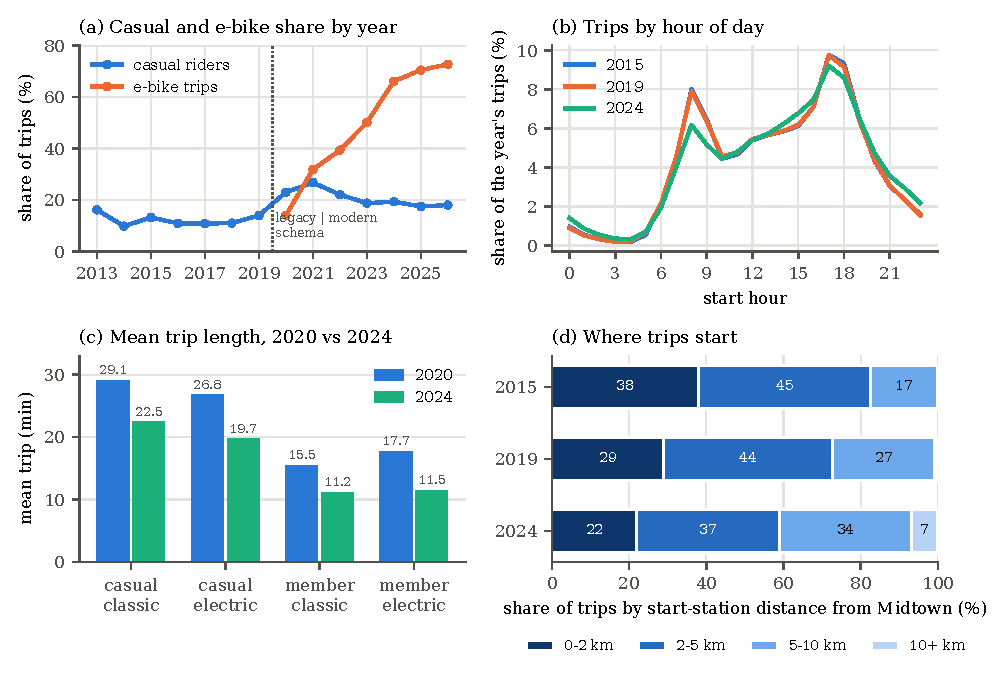
\includegraphics[width=\linewidth]{figures/results.pdf}
\caption{Results from the published Gold tables. In panel (a), casual riders before 2020 are the legacy type Customer and
from 2020 on the modern type casual. Panel (d) uses the distance of the start station from Times Square.}
\label{fig:results}
\end{figure}

\subsection{Casual riders}

The share of casual riders was 13.2\,\% in 2015 and 14.0\,\% in 2019. It jumped to 23.0\,\% in 2020, peaked at 26.7\,\% in
2021 and fell back to 19.3\,\% in 2024 (Figure~\ref{fig:results}a). The pandemic therefore brought a lasting increase, but
about half of the jump has faded since. Because the definition of a casual rider changes with the schema, part of the step
from 2019 to 2020 may come from the definition. The trend from 2020 to 2024 uses only one definition.

\subsection{Electric bikes}

The share of trips on electric bikes grew from 14\,\% in 2020 to 66\,\% in 2024 and 73\,\% in 2026. Since 2023 most trips
are electric. The mean trip length rose from 14.3 minutes in 2019 to 18.8 minutes in 2020 and fell to 13.2 minutes in 2024.
The effect of the electric bike depends on the rider type (Figure~\ref{fig:results}c). In 2024 casual riders were about three
minutes faster on an electric bike, with 19.7 compared to 22.5 minutes. Members rode about equally long on both, with 11.5
compared to 11.2 minutes. Members therefore seem to use the electric bike to ride farther rather than to arrive earlier.

\subsection{Daily peaks}

The evening peak at 17:00 stayed the same. The morning peak became weaker: the hour from 8:00 carried 8.0\,\% of all trips
in 2015, 7.9\,\% in 2019 and only 6.2\,\% in 2024, while the early afternoon and the evening gained
(Figure~\ref{fig:results}b). This fits with more flexible working hours after the pandemic.

\subsection{Distance from central Manhattan}

The share of trips that start within 2~km of Midtown fell from 38\,\% in 2015 to 29\,\% in 2019 and 22\,\% in 2024. In the
same time the share of trips that start more than 5~km away grew from 17\,\% to 41\,\% (Figure~\ref{fig:results}d). The five
busiest stations, however, are still within 3~km of Midtown in all three years, with one exception in 2024 at a distance of
5.1~km. Most of this shift comes from the growth of the network into Brooklyn, Queens and the Bronx, from 471 start stations
in 2015 to more than 2,200 in 2024. The measure therefore shows where the system reaches more than a change in behaviour.

\subsection{Answer to the question}

Both events changed how New Yorkers use Citi Bike. The pandemic left a higher share of casual riders and a weaker morning
peak. Electric bikes became the normal choice within four years. Use also spread out from central Manhattan, but mostly
because the network itself grew.

% ---------------------------------------------------------------------------------------------
\section{Limitations and reflection}

\subsection{Limitations}

Legacy data has no bike type, so all legacy trips are counted as classic, and it defines rider types differently. One case
of daylight saving time cannot be detected (Section~\ref{sec:dst}). The shift away from Midtown is mixed with the growth of
the network, and a fairer comparison would only use stations that existed in all three years. The performance numbers come
from one or two runs on shared virtual machines, and the change to the Silver write was not repeated on the full history.
Finally, the NFS server and the driver run on the same node, which makes it a single point of failure.

\subsection{Reflection}

Four lessons stand out. First, profiling everything before writing rules pays off. A sample led me to wrong timestamp rules,
while the full profile took less than eight minutes. Second, a decision should be stored in a column at the moment it is
made, because deriving it later from data that has already changed caused the bug in the daylight saving repair. Third, the
event log should be read before forming a hypothesis. Two of my four performance hypotheses were wrong, and each time the
event log showed why. Fourth, the accounting checks in every layer were the most useful quality measure. Bronze is checked
against the manifest, Silver must balance and Gold must match Silver. These checks turned a result that looks right into a
check that fails the run when it is not.

With more time I would compare only stations that exist in all core years, join weather data for Central Park to separate
the weather from changes in behaviour, and build Gold incrementally instead of fully every month.

\end{document}
